\section{3. Testbed description}
\textnormal{
	\hspace*{1cm}Doing Researches require proper testing environment, which is able to run required test-cases and is relatively comfortable to use.
	The vital thing is that the results must be reliable and can give desired conclusions about particular problems. In this case ns-3 simulator has been chosen. This chapter focuses on an overview of this tool and scenario prepared using it.}
\subsection{\hspace*{1cm} 3.1 Overview of the ns-3 simulator}
\textnormal{
	\hspace*{1cm}Ns-3 simulator is an open source tool written in C++ programming language with bindings available for Python.It is targeted primarily for research and educational use and is under license of GNU GPLv2. Ns-3 is a discrete-event simulator, so models the operation of a system as a discrete sequence of events in time. Interface of this tool are files with extension of 'cc' or 'py', so models and simulations are directly written in C++ or Python programming languages. Simulation's events are executed in order which is determined by scheduler and the simulation stops when all of the events finish. There is a documentation for ns-3 available on it's official page as well as many scripts and examples. The only operating system which is supported by ns-3 is a Linux. During writing of the thesis 'Ubuntu 16.0.54 LTS' version was used and the version of simulator was 3.29.}
\subsection{\hspace*{1cm}3.2 Scenario description}
	\textnormal{\hspace*{2cm}In order to research specified in the title of the thesis, the particular scenario has been configured. The conditions of simulation's were dynamically changing so automation was needed to run simulation relatively fast and without additional manual chcnages in test scenario. There were separated tools involved to observe specific behaviours and analyze results like statistics libraries of python and wireshark. Everything had to be done in a proper order starting from configuring the scenario, writing automation script and proceeding and analyze essential data produced in time of simulation.}
\subsubsection{\hspace*{1cm}3.2.1 Topology}
	\textnormal{\hspace*{1cm}Topology consists of two wireless Access Points. The first one is to receive traffic from slow stations and the second one from fast stations. Slower stations send data with much lower rate. Simulation scenario includes those 2 types of stations to observe different explore how stations with completely different data rates behave when it comes to share frequency range with LTE signals. There are also cases where there is  only one Access Point. The number of stations is variable and can be changed whenever it is needed also while simulation is running. Each staion send data to it's own access point.\newline\hspace*{1cm}Essential part of the topology is an interferer which is configured to act as a LTE base station and generate signals which interfere with 802.11 transmission. In some scenarios Interferer must be excluded so and then it's transmit power is decreased to zero. Basic Topology is shown in Figure 3.1. }
	\begin{figure}[h]
	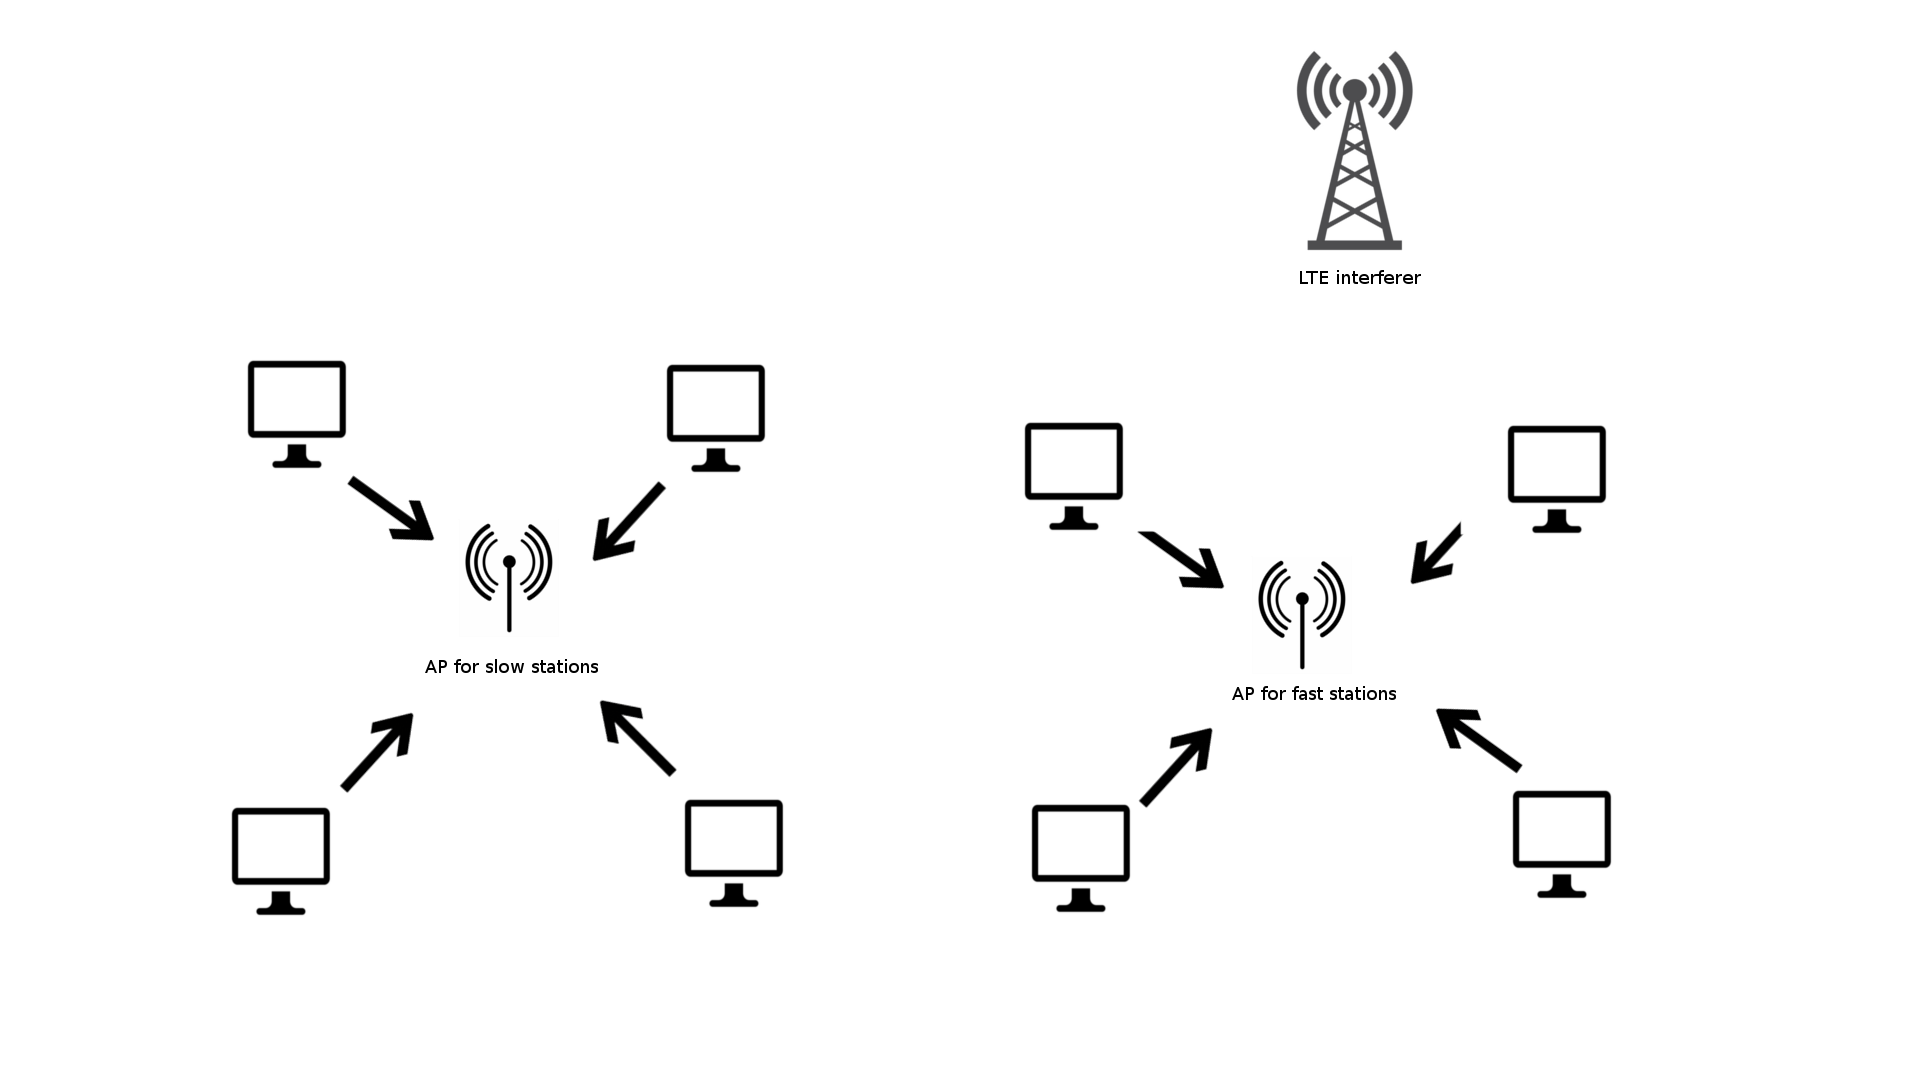
\includegraphics[scale=0.25]{Images/topology}
	
	\caption{Basic Topology}
	\end{figure}
\subsubsection{3.2.2 Code description}
\subsubsection{3.2.3 Input parameters}
\subsubsection{3.2.4 Flow Monitor}
\subsubsection{3.2.5 Simulation Automation}
